\documentclass{beamer}
\usepackage[utf8]{inputenc}
\usepackage{graphicx}
\usepackage{hhline}
\usepackage{pdfpages}
\usepackage{subcaption}
\usepackage[demo]{graphicx}
\usepackage{makecell}
\usepackage[mode=buildnew]{standalone}
\usepackage{amsmath}
\usepackage{mathtools}
\usepackage{tikz}
\usepackage{environ}
\usepackage{fontawesome}
\usepackage{caption}
\usepackage[backend=bibtex,style=authoryear-comp,dashed=false,natbib=true]{biblatex}
\addbibresource{bibtex.bib}
% \setbeamertemplate{footline}[frame number]
\setbeamerfont{footnote}{size=\Tiny}
\setlength\bibitemsep{1.5\itemsep}
\graphicspath{{img/}}
\setbeamertemplate{navigation symbols}{}
\setbeamertemplate{page number in head/foot}{}
\setbeamertemplate{bibliography item}{}
\setbeamertemplate{caption}[numbered]
\setbeamercovered{transparent}
\renewcommand\refname{Bibliography}
\setbeamerfont{institute}{size=\small}
\usetheme{Frankfurt}
\usecolortheme{whale}
\DeclareMathOperator*{\argmax}{argmax} 
\DeclareCaptionFormat{myformat}{\fontsize{6}{6}\selectfont#1#2#3}
\captionsetup{format=myformat}
\captionsetup[figure]{labelfont={bf},name={Figure}}
\captionsetup[table]{labelfont={bf},name={Table}}
\renewcommand{\arraystretch}{1.3}

\newcommand{\customframefont}[1]{
	\setbeamertemplate{itemize/enumerate body begin}{#1}
	\setbeamertemplate{itemize/enumerate subbody begin}{#1}
}

\NewEnviron{framefont}[1]{
	\customframefont{#1} % for itemize/enumerate
	{#1 % For the text outside itemize/enumerate
		\BODY
	}
	\customframefont{\normalsize}
}

\setbeamertemplate{footline}{% 
	\hfill% 
	\usebeamercolor[fg]{page number in head/foot}% 
	\usebeamerfont{page number in head/foot}% 
	\insertframenumber%
	%\,/\,\inserttotalframenumber
	\kern1.2em\vskip4.5pt% 
}

\renewcommand\cellgape{\Gape[3pt]}
\definecolor{ao(english)}{rgb}{0.0, 0.5, 0.0}

\title{Mining Sentiments and Arguments in United
Nations Security Council (UNSC) Speeches}
\subtitle{"Exploring the UNSC political speech corpus"}
\author{Atreya Shankar, Juliane Hanel \\ Cognitive Systems (M.Sc.)}
\institute{PM: Mining Sentiments and Arguments \\ University of Potsdam, WiSe 19/20 \\ Prof. Dr. Manfred Stede}
\date{February 4. 2020}

\begin{document}
	\begin{frame}
		\maketitle
	\end{frame}
	
	\begin{frame}
		\frametitle{Table of Contents}
		\setbeamertemplate{enumerate items}[square]
		\begin{enumerate}
			\setlength\itemsep{1em}
			\item Recap
			\item Sentiment Analysis
			\item Argumentation Mining
			
			\item Bibliography
		\end{enumerate}
	\end{frame}
	
\section{Recap}

	\subsection{}
	\begin{framefont}{\footnotesize}
		\begin{frame}
			\frametitle{Recap: Objectives}
			\begin{itemize}
				\setlength\itemsep{1.5em}
				\item \textbf{General objective:} Explore mining various components of the UNSC political speech corpus
				\item \textbf{Approach 1:} Using sentiment and subjectivity analysis
				\item \textbf{Approach 2:} Mining argumentation structure of speeches
			
			\end{itemize}
		\end{frame}
	\end{framefont}

	\subsection{}
	\begin{framefont}{\footnotesize}
		\begin{frame}
			\frametitle{What have we achieved so far?}
			\begin{itemize}
				\setlength\itemsep{1.2em}
				\item \textbf{Data preparation:} Organizing more than 65k unprocessed speeches including metadata
				\item \textbf{Research:} Wrapping our heads around state-of-the-art methods
				\item \textbf{Coding:} Implementing fundamental ideas and prototypes
				\item \textbf{Realizations:} How feasible are our objectives? 
			\end{itemize}
		\end{frame}
	\end{framefont}
	
	

	
	

\section{Sentiment Analysis}	



\subsection{}
\begin{framefont}{\footnotesize}
	\begin{frame}
		\frametitle{Sentiment Analysis - Methodologies}


	
		\textbf{Sentiment Analysis:}
		\begin{itemize}
			\setlength\itemsep{0.8em}
			\item \textit{Vader} for comparative sentiment analysis ([-1,1] from negative over neutral to positive)
			\item \textit{TextBlob} did not perform well, a joint approach of the two frameworks is not feasible
		\end{itemize}
			
		
		\textbf{Subjectivity Analysis:}	 
        \begin{itemize}
        \item \textit{TextBlob} for subjectivity analysis ([0,1] from objective to subjective)
        \item Possible extension with \textit{MPQA} subjectivity lexicon \citep{mpqa}
		\end{itemize}
		
	
	\end{frame}
\end{framefont}



\subsection{}
\begin{framefont}{\footnotesize}
	\begin{frame}
		\frametitle{Sentiment Analysis}
		
		\begin{figure}[htb]
    \centering
    \begin{subfigure}[b]{\textwidth}
        \centering
        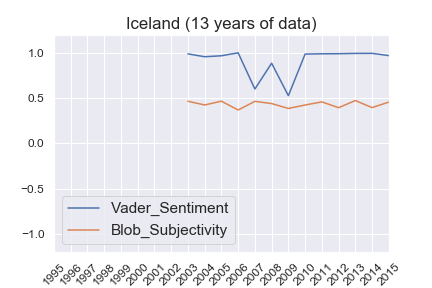
\includegraphics[width=0.475\linewidth]{iceex.png}%
        \hfill
        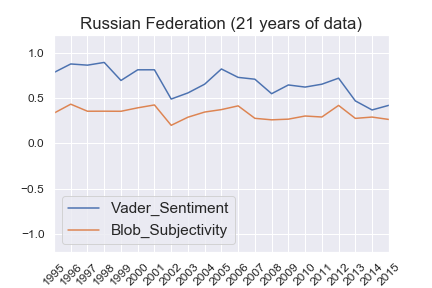
\includegraphics[width=0.475\linewidth]{russiaex.png}
        
    \end{subfigure}
    \vskip
    \begin{subfigure}[b]{\textwidth}
        \centering
        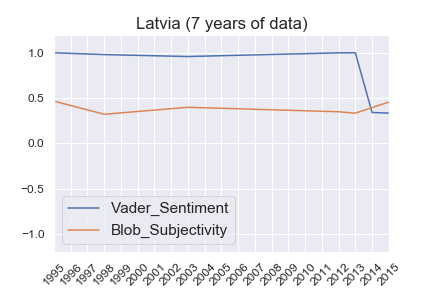
\includegraphics[width=0.475\linewidth]{latvex.png}%
        \hfill
        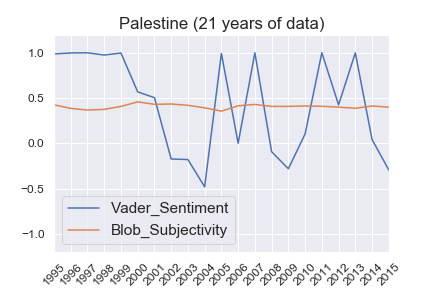
\includegraphics[width=0.475\linewidth]{palex.png}
        
    \end{subfigure}
    \caption{Examples of the sentiment analysis \\
    \textbf{$\longrightarrow$ What is worth investigating?}}
    
\end{figure}

	\end{frame}
\end{framefont}


\subsection{}
\begin{framefont}{\footnotesize}
	\begin{frame}
		\frametitle{Example - Core Nations}
		
		
		
		\begin{figure}
					\captionsetup{justification=centering}
					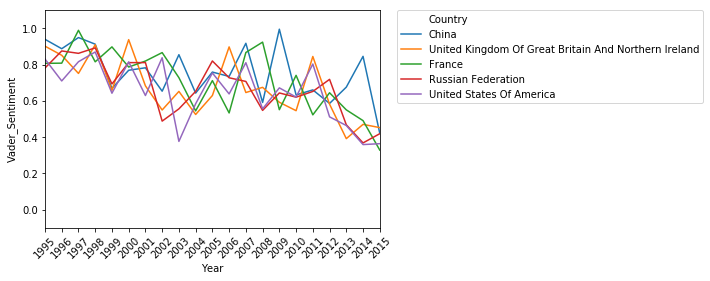
\includegraphics[trim={0cm 0cm 0cm 0.2cm},clip,width=11.5cm]{vadercore.png}
					\caption{Sentiment of the UNSC core nations over time}
			\end{figure}
			
		
	
	\end{frame}
\end{framefont}


\subsection{}
\begin{framefont}{\footnotesize}
	\begin{frame}
		\frametitle{Example - Core Nations}
		
		\textbf{What is worth investigating?}
		
		\begin{figure}
					\captionsetup{justification=centering}
					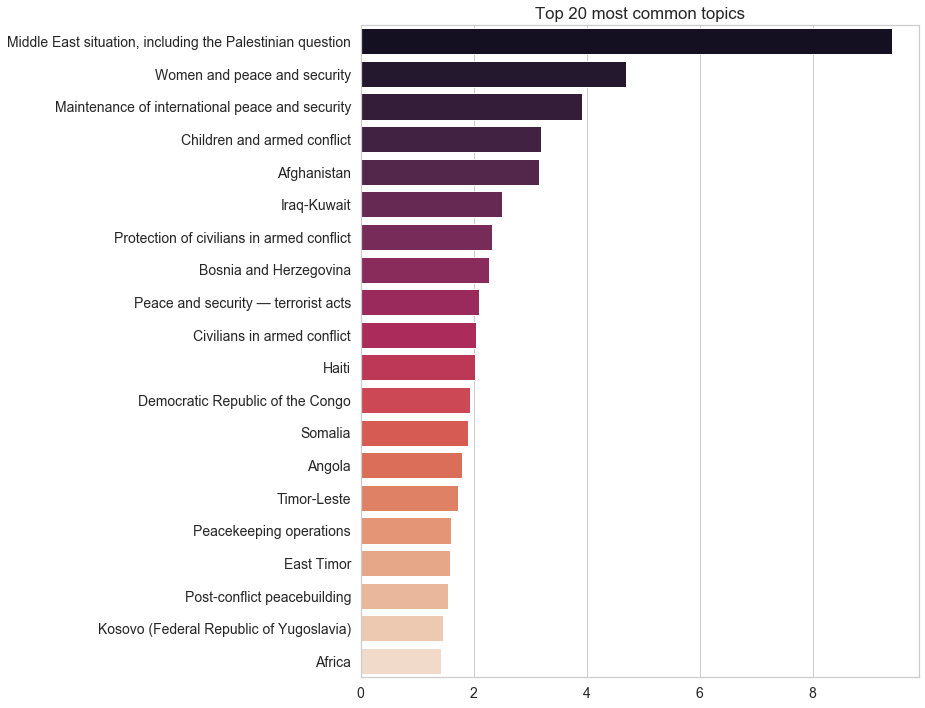
\includegraphics[trim={0cm 0cm 0cm 0cm},clip,width=9cm]{20most_common_topics.png}
					\caption{Relative frequency of topics (overall)}
			\end{figure}
		
	
	\end{frame}
\end{framefont}



\subsection{}
\begin{framefont}{\footnotesize}
	\begin{frame}
		\frametitle{Example - Core Nations}
		
		
		
		\begin{figure}
					
					
					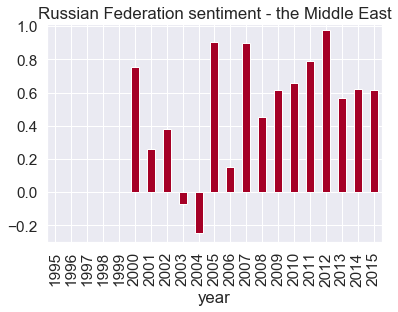
\includegraphics[trim={0.3cm 0cm 0cm 0.2cm},clip,width=7cm]{Russian_Federation.png}
					\caption{Russia as example for the sentiment in core nation \\speeches concerning the Middle East situation}
			\end{figure}
			$\longrightarrow$ 2002: \textit{Road map for peace} was founded
	
	\end{frame}
\end{framefont}

\subsection{}
\begin{framefont}{\footnotesize}
	\begin{frame}
		\frametitle{Evaluation?}
	%%% make this slide prettier, is it still possible to read the text when they're next to each other??	
	\begin{table}[]
\begin{tabular}{c|c|}
\hline
\multicolumn{1}{|c|}{\textbf{Positive Words}} & \textbf{Negative Words} \\ \hline
\multicolumn{1}{|c|}{important}               & conflict                \\ \hline
\multicolumn{1}{|c|}{urgent}                  & dangerous               \\ \hline
\multicolumn{1}{|c|}{acceptable}              & confrontation           \\ \hline
\multicolumn{1}{|c|}{support}                 & stop                    \\ \hline
                                              & violence                \\ \cline{2-2} 
\end{tabular}
\end{table}

		\begin{figure}
					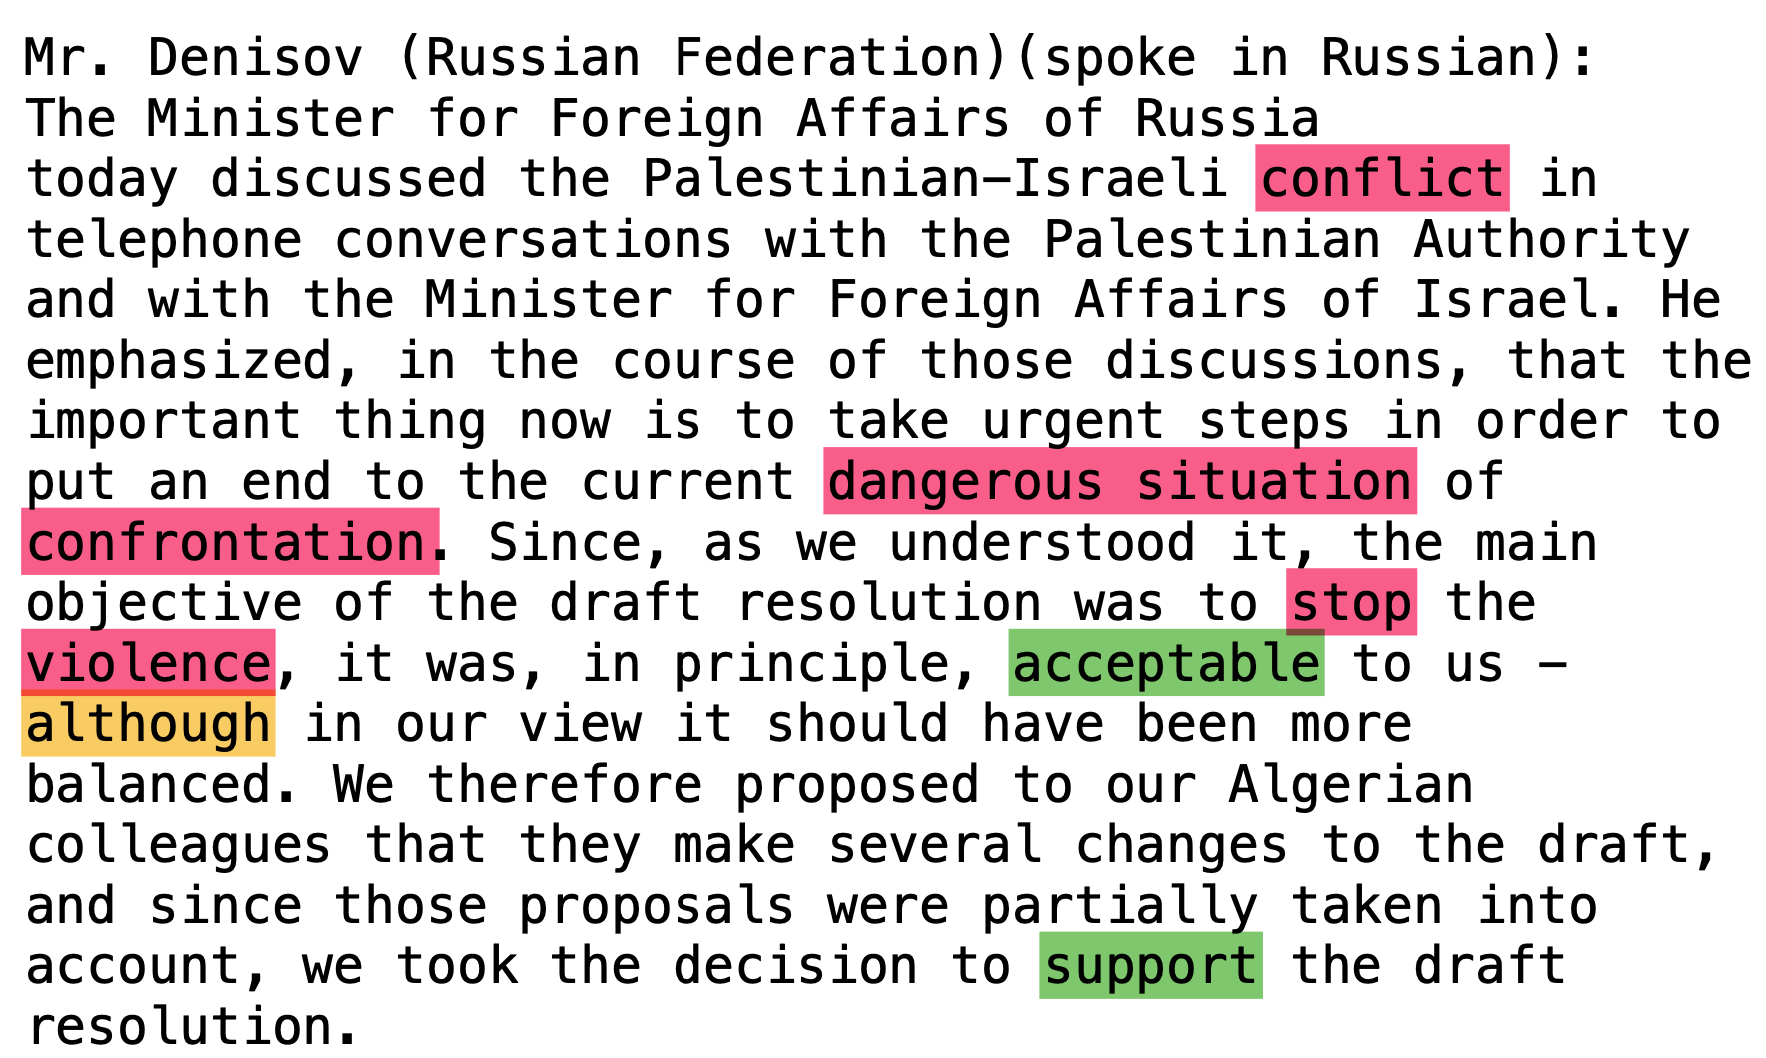
\includegraphics[trim={0cm 0cm 0cm 0cm},clip,width=6cm]{russia_manual.png}
					\caption{Relevant words in Vader vs. manual sentiment annotation}
			\end{figure}
			
	
	\end{frame}
\end{framefont}





\subsection{}
\begin{framefont}{\footnotesize}
	\begin{frame}
		\frametitle{Further Steps}
		\begin{itemize}
			\setlength\itemsep{1.2em}
			\item Deciding on evaluation method (Words, sentences, speeches? One or multiple opinions?)
			
			\item Deciding on the analysis scope (Core nations? Specific topics?) 
			\item Improving performance of subjectivity analysis by integrating lexica
			\item Organizing and implementing the final ideas
			
			
		\end{itemize}
	\end{frame}
\end{framefont}

\section{Argumentation Mining}
\subsection{}
\begin{framefont}{\footnotesize}
	\begin{frame}
		\frametitle{Recap: Argumentation Mining}
			\begin{figure}				       
			\captionsetup{justification=centering}
		   	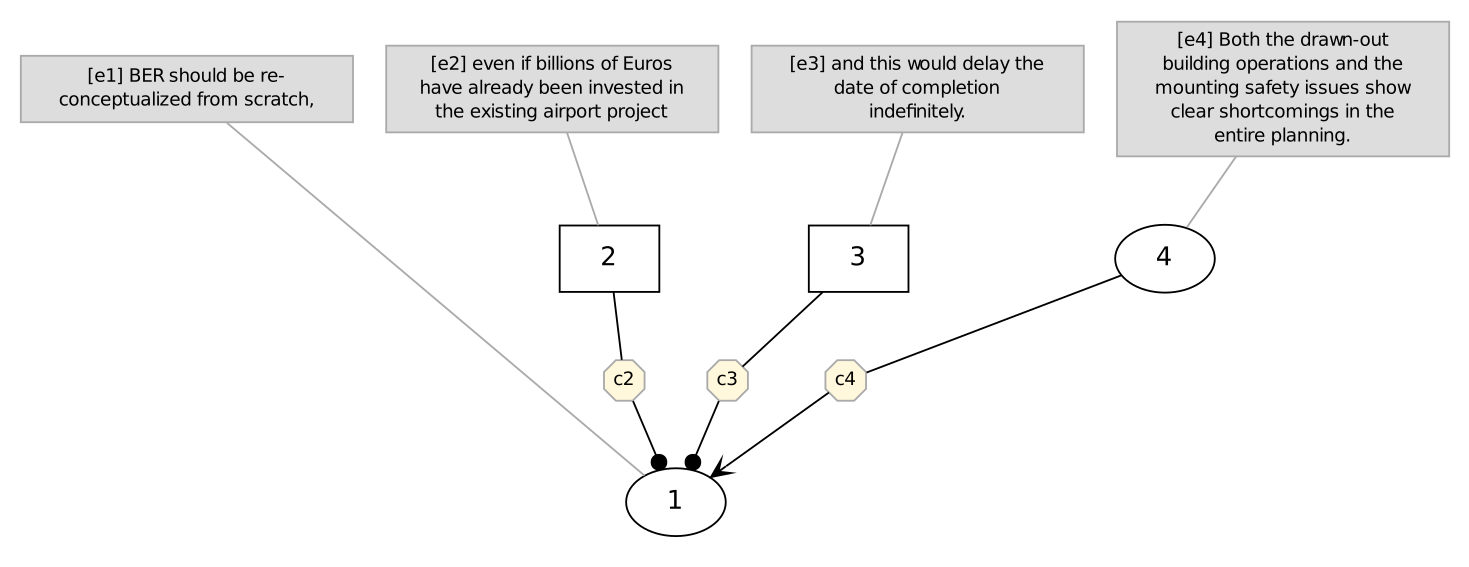
\includegraphics[trim={0cm 0cm 0cm 0cm},clip,width=8cm]{args_structure.png}
		   	\caption{Example of a complete argumentative structure of a short text \citep{peldszus2015annotated}}
			\end{figure}
		\begin{itemize}
			\setlength\itemsep{0.8em}
			\item Argumentation structure requires claims and premises; which are usually assembled into a tree structure
			\item Specify support/attack nature of claims and premises; \textit{omitted in our project}
			\item Train argumentation classifier on US Election Debate corpus, apply on UNSC corpus
		\end{itemize}
	\end{frame}
\end{framefont}

\subsection{}
\begin{framefont}{\footnotesize}
	\begin{frame}
		\frametitle{US Election Debate Corpus}
			\begin{columns}
				\column{0.40\linewidth}
				\begin{figure}
				    \centering
					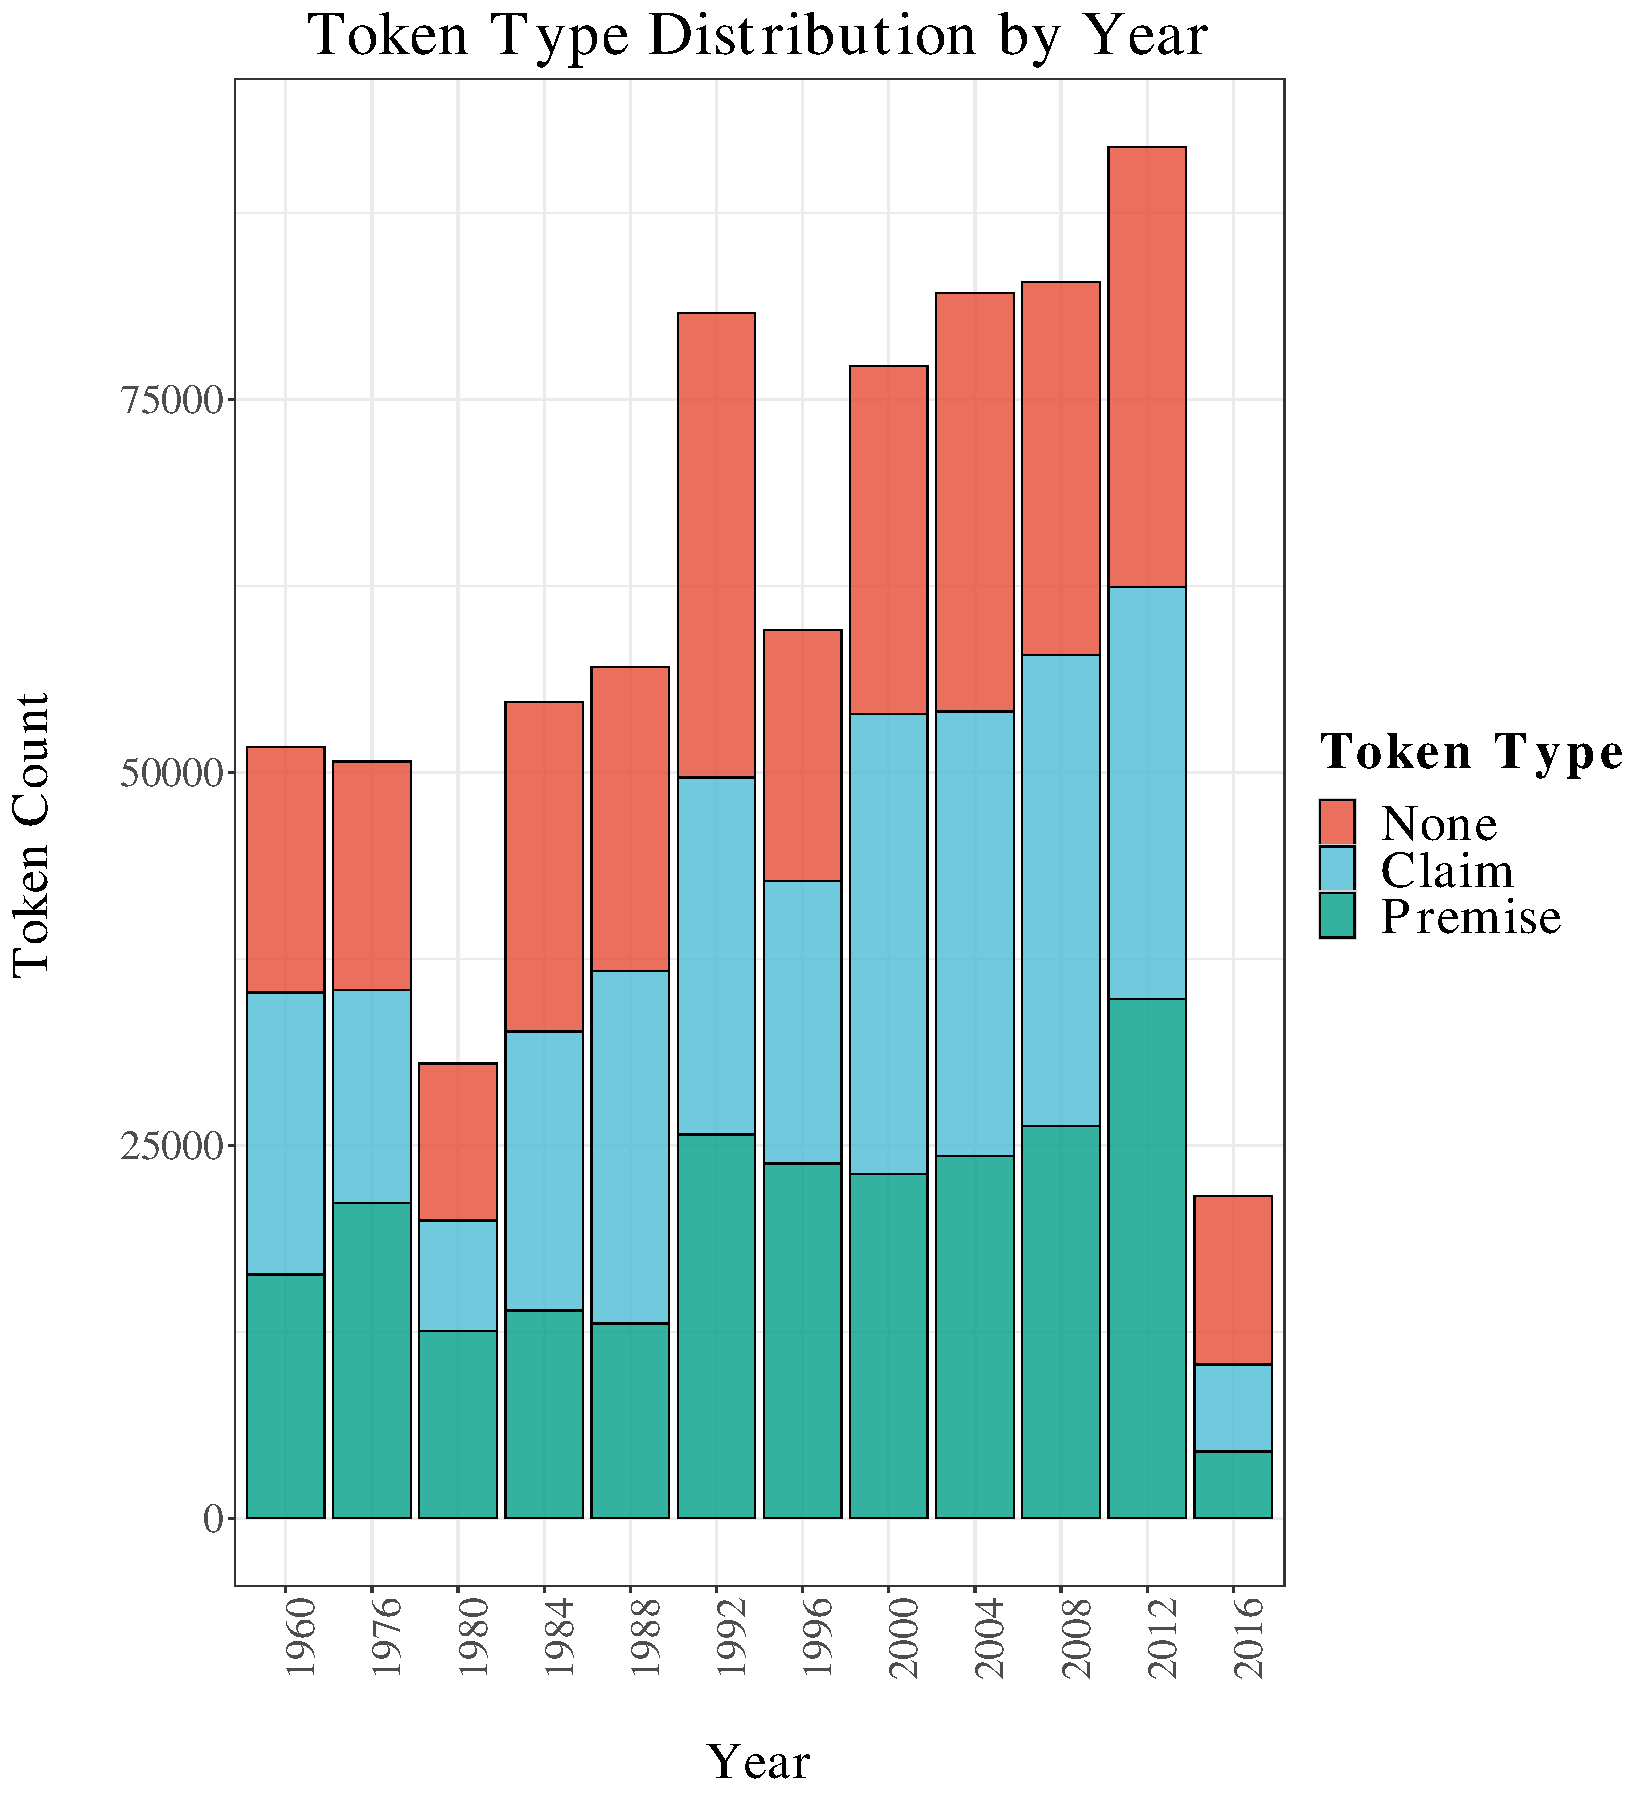
\includegraphics[trim={0.05cm 0.05cm 0.05cm 0.05cm},clip,width=5.3cm]{global.pdf}
					\captionsetup{justification=centering,margin={0.6cm,0cm}}
					\caption{Token type distribution in the US election debate corpus by year}
				\end{figure}
				\column{0.003\linewidth}
				\column{0.60\linewidth}
				\begin{itemize}
					\setlength\itemsep{1.5em}
					\item US election debate corpus consists of 42 annotated presidential debate sessions from 1960 until 2016 \citep{haddadan-etal-2019-yes}
					\item Pre-processing of character spans yields token-based annotations
					\item Tokens can either be of class "None" (N), "Claim" (C) or "Premise" (P)
					\item \textbf{Task 1} $\Longrightarrow$ sequence tagging of tokens to N, C or P
					\item \textbf{Task 2} $\Longrightarrow$ argumentation structure via adjacency matrix
				\end{itemize}
			\end{columns}
	\end{frame}
\end{framefont}

\subsection{}
\begin{framefont}{\footnotesize}
	\begin{frame}
		\frametitle{(AL)BERT as Input Encoder}
			\begin{columns}
				\column{0.40\linewidth}
				\begin{figure}
				    \centering
					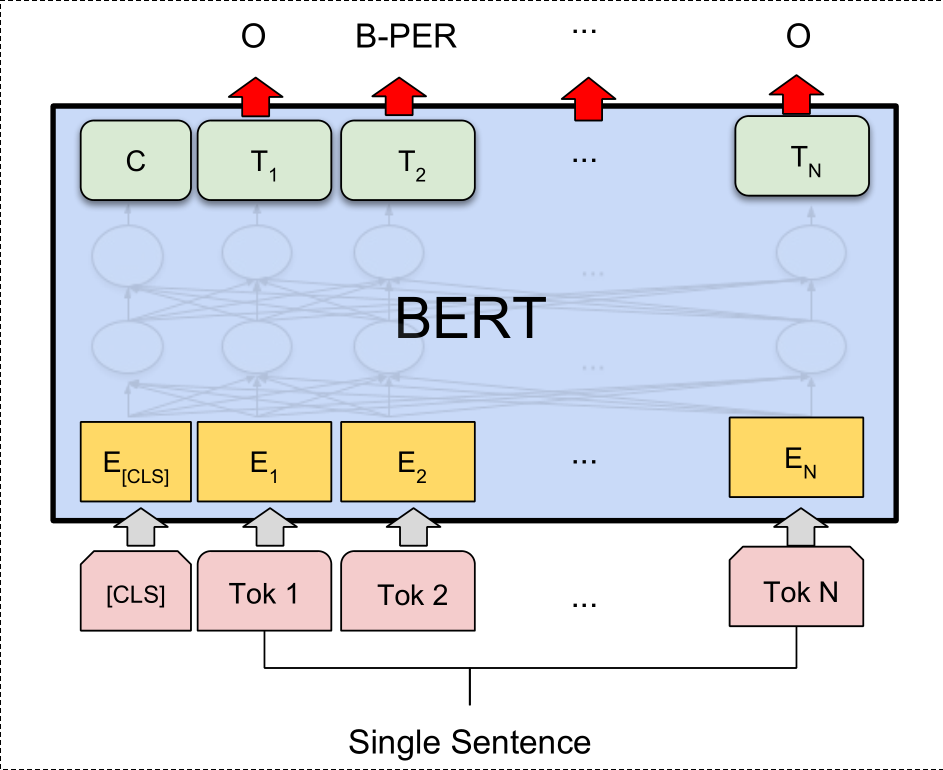
\includegraphics[trim={0.2cm 0.2cm 0.2cm 0.2cm},clip,width=5.3cm]{bert.png}
					\captionsetup{justification=centering,margin={0.5cm,-0.7cm}}
					\caption{Sample schematic of using BERT for Natural Entity Recognition (NER) task \citep{devlin2018bert}}
				\end{figure}
				\column{0.01\linewidth}
				\column{0.60\linewidth}
				\begin{itemize}
					\setlength\itemsep{1.0em}
					\item \textbf{B}idirectional \textbf{E}ncoder \textbf{R}epresentations from \textbf{T}ransformers (BERT) and its variants have shown SOTA performance on various NLP tasks \citep{devlin2018bert}
					\item BERT$_{\text{base}} \Longrightarrow \quad \sim 108$M parameters
					\item Unrealistic to fine-tune on single NVIDIA GeForce GTX 1080 Ti with 12 GB RAM (Uni-Potsdam available hardware)
					\item Alternative is the "Lite" version of BERT, known as ALBERT \citep{lan2019albert}
					\item ALBERT$_{\text{base}} \Longrightarrow \quad \sim 12$M parameters
					\item $O(N^2)$ space complexity wrt. sequence length for attention mechanism
				\end{itemize}
			\end{columns}
	\end{frame}
\end{framefont}

\subsection{}
\begin{framefont}{\footnotesize}
	\begin{frame}
		\frametitle{US Election Debate Corpus Pruning}
			\begin{figure}				       
			\captionsetup{justification=centering}
		   	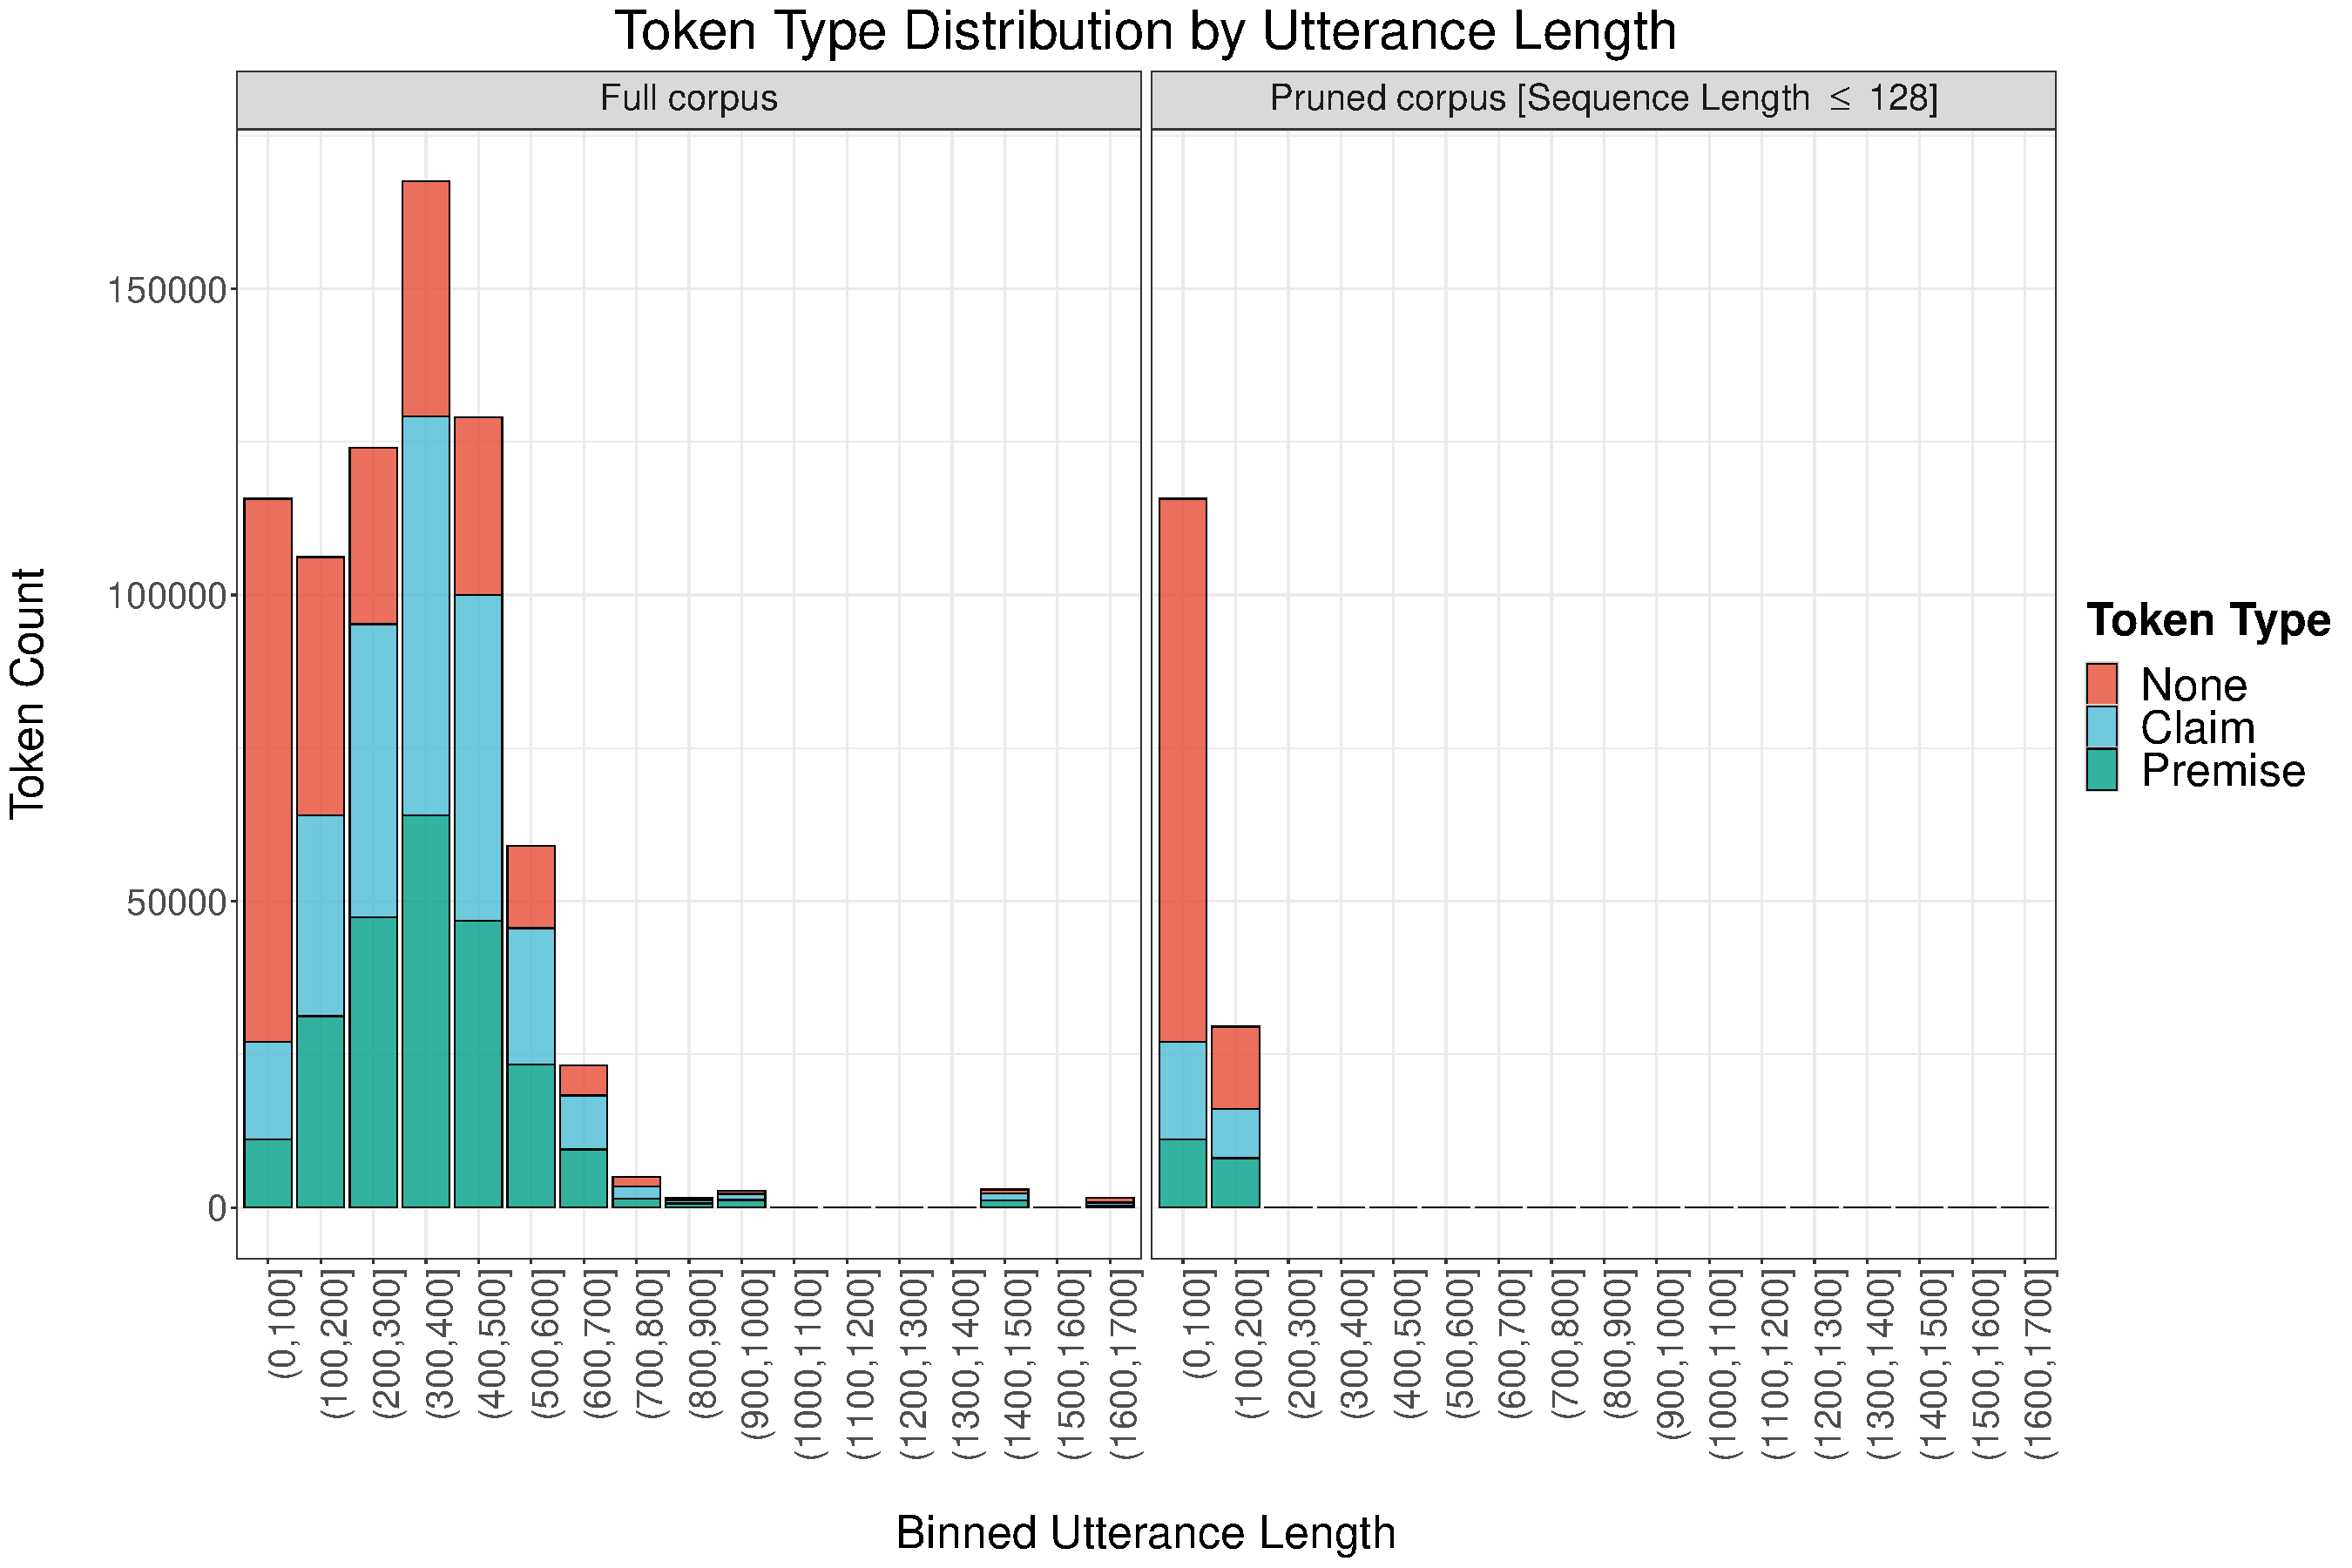
\includegraphics[trim={0cm 0cm 0cm 0cm},clip,width=9cm]{global_length_trunc.pdf}
		   	\caption{Token type distributions based on binned utterance length; based on full (left) and pruned corpus (right)}
			\end{figure}
		\vspace{-3pt}
		\begin{itemize}
			\setlength\itemsep{0.8em}
			\item Keep sequences where N$_{\text{tokens}} \leq 128$; corpus size reduced from 6559\\ $\longrightarrow$ 4594 utterances
		\end{itemize}
	\end{frame}
\end{framefont}

\subsection{}
\begin{framefont}{\footnotesize}
	\begin{frame}
		\frametitle{Fine-tuning ALBERT}
			\begin{columns}
				\column{0.003\linewidth}
				\column{0.40\linewidth}
				\begin{figure}
				    \centering
					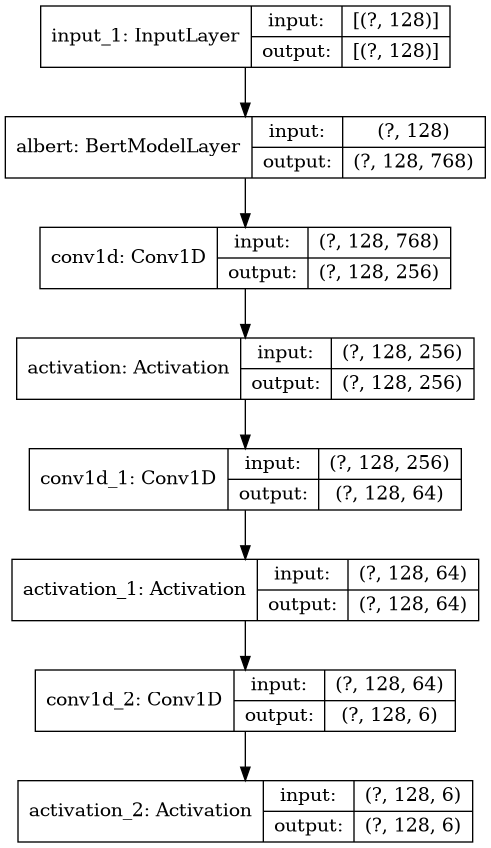
\includegraphics[trim={0cm 0cm 0cm 0cm},clip,width=3.5cm]{model.png}
					\captionsetup{justification=centering}
					\caption{Sample graph for ALBERT encoder with 1D-Convolution decoder}
				\end{figure}
				\column{0.60\linewidth}
				\begin{itemize}
					\setlength\itemsep{1.2em}
					\item To fine-tune ALBERT on the argument classification task, we must decode ALBERT output to our supervised output
					\item The following architectures were tested through a grid-search with various learning profiles and normalization techniques; albeit with a fixed batch size of \textit{48} to prevent OOM issues
					\item[i.] 3 layer time-distributed dense (TD-Dense)
					\item[ii.] 3 layer fully 1D-Convolutional (1D-Conv)
					\item[iii.] 2 layer LSTM decoder (Stacked-LSTM)
				\end{itemize}
			\end{columns}
	\end{frame}
\end{framefont}

\subsection{}
\begin{framefont}{\footnotesize}
	\begin{frame}
		\frametitle{Model Performance on Task 1 (Sequence Tagging)}
    \begin{table}[]
    \begin{tabular}{|l|l|l|l|l|l|}
    \cline{1-6}
    Model & Train F$_1$ & Test F$_1$ & Test F$_1$[N] & Test F$_1$[C] & Test F$_1$[P]\\ \hhline{|=|=|=|=|=|=|}
    \textbf{TD-Dense} & 0.674 & \textbf{0.643} & 0.917 & 0.5174 & \textbf{0.495} \\ \cline{1-6}
    1D-Conv & 0.744 & 0.610 & 0.899 & 0.513 & 0.419 \\ \cline{1-6}
    Stacked-LSTM & 0.609 & 0.629 & 0.899 & \textbf{0.569} & 0.419 \\ \cline{1-6}
    \end{tabular}
    \caption{Model performance summary based on train and test set F$_1$ scores}
    \end{table}
    \begin{itemize}
    	\setlength\itemsep{0.8em}
        \item Similar performances with $\sim 60 \%$ F$_1$ scores on test set
        \item High F$_1$ scores across N-token classification, as it is a majority class
        \item TD-Dense shows the best overall performance; with best performance in P-token classification
        \item Stacked-LSTM has second-best overall performance; with best performance in C-token classification
    \end{itemize}
	\end{frame}
\end{framefont}

\subsection{}
\begin{framefont}{\footnotesize}
	\begin{frame}
		\frametitle{Further steps}
		\begin{enumerate}
		\setbeamertemplate{enumerate items}[square]
			\setlength\itemsep{1.2em}
			\item To prevent data loss from corpus pruning, use gradient accumulation in optimizers \footnote{https://github.com/run-ai/runai} to allow for smaller local batch-sizes and potentially longer sequence lengths; without affecting global batch-sizes
			\item Improve train/test/validation data splits to be representative of overall corpus
			\item Develop graph neural network to create explicit argumentation structure from annotated tokens $\Longrightarrow$ hypothesis is that multi-task setting will improve performances of both tasks
			\item Run best classifier on short sequences in UNSC corpus to manually grade performance
		\end{enumerate}
	\end{frame}
\end{framefont}

\begin{frame}[allowframebreaks]
	\frametitle{Bibliography}
	\nocite{*}
	\printbibliography[title = {Bibliography}]
\end{frame}

\end{document}